\documentclass[12pt,a4paper]{article}
\usepackage[utf8]{inputenc}
\usepackage[T1]{fontenc}
\usepackage{amsmath,amssymb,amsfonts}
\usepackage{epsfig,color}
\usepackage[svgnames]{xcolor}
\usepackage{tikz}
\usepackage{enumitem,colortbl}
\usepackage{adjustbox,pifont,amssymb}
\usepackage[citecolor=blue,urlcolor=blue,unicode=true,pdfusetitle, bookmarks=true,bookmarksnumbered=true,bookmarksopen=true,bookmarksopenlevel=3, breaklinks=false,pdfborder={0 0 1},backref=false,colorlinks=true, linkcolor=blue]{hyperref}
\usetikzlibrary{arrows,arrows.meta,shapes,positioning,shadows,trees,calc,intersections,external}

\begin{document}

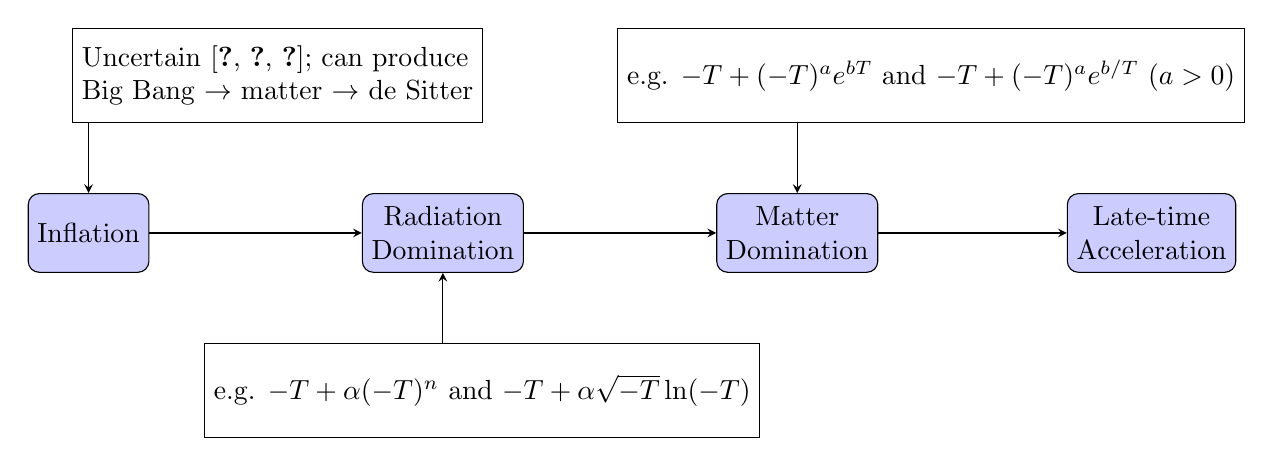
\begin{tikzpicture}[node distance=1.5cm, >=stealth,
	topic/.style={align=center,rectangle,minimum height=10mm,draw,rounded corners,fill=blue!20},
	subtopic/.style={rectangle,draw,minimum size=35mm,minimum height=12mm}]
	\node[topic] (infl) {Inflation};
	\node[topic, right of = infl, xshift = 3cm] (rad) {Radiation \\ Domination};
	\node[topic, right of = rad, xshift = 3cm] (matt) {Matter \\ Domination};
	\node[topic, right of = matt, xshift = 3cm] (acc) {Late-time \\ Acceleration};
	\node[subtopic, align = justify, above of = infl, xshift = 2.4cm, yshift = 0.5cm] (infl-models) {Uncertain \cite{Wu:2010xk,Mirza:2017vrk,Hohmann:2017jao}; can produce \\ Big Bang $\to$ matter $\to$ de Sitter};
	\node[align = center, subtopic, xshift = 0.5 cm, yshift = -0.5cm, below of = rad] (rad-models) {e.g. $-T + \alpha (-T)^n$ and $-T + \alpha \sqrt{-T} \ln (-T)$};
	\node[subtopic, align = justify, above of = matt, xshift = 1.7cm, yshift = 0.5cm] (matt-models) {e.g. $-T + (-T)^a e^{bT}$ and $-T + (-T)^a e^{b/T}$ $(a > 0)$};
	\draw[->] (infl) -- (rad);
	\draw[->] (rad) -- (matt);
	\draw[->] (matt) -- (acc);
	\draw[->] ([xshift=-2.4cm]infl-models.south) -- (infl);
	\draw[->] ([xshift=-0.5cm]rad-models.north) -- (rad);
	\draw[->] ([xshift=-1.7cm]matt-models.south) -- (matt);
	\end{tikzpicture}

\end{document}